\documentclass[12pt]{article}
\usepackage[a4paper,
            bindingoffset=0.2in,
            left=0.79in,
            right=0.79in,
            top=0.79in,
            bottom=0.79in,
            footskip=.25in]{geometry}
% Les packages

\usepackage[french]{babel}
\usepackage[T1]{fontenc}
\usepackage[utf8]{inputenc}

\usepackage{geometry}
\usepackage{fancyhdr}
\pagestyle{fancy}
\usepackage{csquotes}

\usepackage{ amssymb }
\usepackage{etoolbox}
\fancyhf{} % Clear header/footer
\makeatletter
%\patchcmd{\f@nch@head}{\rlap}{\color{red}\rlap}{}{}
\patchcmd{\headrule}{\hrule}{\color{black}\hrule}{}{}
%\patchcmd{\f@nch@foot}{\rlap}{\color{green}\rlap}{}{}

\makeatother
\fancyfoot[R]{\thepage}
\usepackage{lastpage}
\usepackage{setspace}
\usepackage{lscape}
\usepackage{multicol}
\usepackage{makeidx}
\usepackage{varioref}
\usepackage{titlesec}
\usepackage[style=authoryear]{biblatex}
\setlength{\columnsep}{0.75cm}
\usepackage{pifont}
\usepackage{eurosym}
\usepackage{soul}
\usepackage[normalem]{ulem}
\usepackage{fancybox}
\usepackage{enumerate}
\usepackage{verbatim}
\usepackage{moreverb}
\usepackage{color}

\usepackage{array}
\usepackage{multirow}
\usepackage{tabularx}
\usepackage{longtable}
\usepackage{colortbl}

\usepackage{graphicx}
\usepackage{wrapfig}
\usepackage{picinpar}
\usepackage{epic}
\usepackage{eepic}
\usepackage{afterpage}
\usepackage{rotating}
\usepackage{float}
\usepackage[font=small]{caption}
\usepackage{subcaption}
\usepackage{microtype}

\usepackage{amsmath}
\usepackage{amssymb}
\usepackage{dsfont}
\usepackage{mathrsfs}
\usepackage{ntheorem}
\usepackage{subscript}
\usepackage{calc}
\usepackage{ifthen}
\usepackage{xspace}
\usepackage{adjustbox}
\usepackage[
    colorlinks=true,
    linkcolor=black,    % \ref, \autoref, etc. in black
    citecolor=black,    % \cite in black
    urlcolor=blue       % only URLs in blue
]{hyperref}


%%%%%%%%%%%%%%%%%%%%%%%%%%%%%%%%%%%%%%%%%%%%%%%%%%%%%%%%%%%%%%%%%%%%%%%%%%%%%%%%%%%%%%%%%%%%%%%%%%%%%%%%%%%%%%%%%%%%%%%%%%%%%%%%%%%%%%%%%%%%%%%%%%%%%%%%%%%%%%%%%%%%%%%%%%%%%%%%%%%%%%%%%%%%%%%%%%%%%%%%%%%%%%%%%%%%%%%%%%%%%%%%%%%%%%%%%%%%%%%%%%%%%%%%%%%%%%%%%%%%


% Les commandes

\newcommand{\SUM}{\sum\limits}
\newcommand{\D}{\displaystyle}







%%%%%%%%%%%%%%%%%%%%%%%%%%%%%%%%%%%%%%%%%%%%%%%%%%%%%%%%%%%%%%%%%%%%%%%%%%%%%%%%%%%%%%%%%%%%%%%%%%%%%%%%%%%%%%%%%%%%%%%%%%%%%%%%%%%%%%%%%%%%%%%%%%%%%%%%%%%%%%%%%%%%%%%%%%%%%%%%%%%%%%%%%%%%%%%%%%%%%%%%%%%%%%%%%%%%%%%%%%%%%%%%%%%%%%%%%%%%%%%%%%%%%%%%%%%%%%%%%%%%


% Les environnements
\usepackage{tikz}
\usetikzlibrary{shapes,shadows}
\tikzstyle{abstractbox} = [draw=black, fill=white, rectangle, inner sep=10pt, style=rounded corners]
\tikzstyle{abstracttitle} =[fill=white]

\definecolor{abstract-back}{RGB}{214, 234, 248}
\definecolor{abstract-frame}{RGB}{36, 113, 163}
\usepackage[skins]{tcolorbox}

\tcbset{
    abstractbox/.style={
        enhanced,
        colback=blue!5!white,
        colframe=blue!75!black,
        fonttitle=\Large\bfseries,
        drop shadow={shadow scale=0.9, shadow xshift=1mm, shadow yshift=-1mm}
    }
}

\newtcolorbox{abstractbox}{abstractbox,
    colback=abstract-back, % Background color
    colframe=abstract-frame, % Border color
    fonttitle=\Large\bfseries, % Bold font for the title
    title=Résumé, % Title texts
    boxrule=1mm}% Border width


\makeatletter
\@ifpackageloaded{babel}{%
  \@ifundefined{NoAutoSpaceBeforeFDP}{%
    \newcommand{\nospace}[1]{#1}%
  }{%
    \newcommand{\nospace}[1]{{\NoAutoSpaceBeforeFDP{}#1}}%
  }%
}{%
  \newcommand{\nospace}[1]{#1}%
}
\makeatother

\usepackage[font=small, skip=2pt]{caption}
\usepackage{graphicx}
\usepackage{float}
\usepackage{multicol}
\usepackage{mathtools} 
\usepackage{indentfirst}
\addbibresource{citations.bib}
\usepackage{titlesec}
\renewcommand{\contentsname}{Sommaire}
\usepackage[french]{babel}

\newcommand{\hour}[2]{#1\mathrel{:}#2}
\newcommand{\commandThatFails}{
    \makeatletter \comma@parse{}{} \makeatother
}

\makeatletter
\DeclareRobustCommand{\NoSpaceColon}{\begingroup\catcode`\:=12 \@NoSpaceColon}
\newcommand{\@NoSpaceColon}[1]{#1\endgroup}
\makeatother


%{\newcommand{\nospace}[1]{{\NoAutoSpaceBeforeFDP{}#1}}}
%{\newcommand{\nospace}[1]{#1}}
\makeatother

\begin{document}

\begin{titlepage}

\begin{center}

    \textsc{\LARGE Master 1 Science de l'Océan, de l'Atmosphère et du Climat \\ \vskip1.5cm Rapport de stage}
    \vskip0.4cm
    \textsc{\Large Avril - juin 2025}
\end{center}
\vspace{0.1cm}
\begin{tcolorbox}[
    enhanced,
    width=\textwidth, % use full text width
    height=3.5cm,
    fontupper=\large\bfseries,
    drop fuzzy shadow,
    valign=center,
    colback=white,
    colframe=black,
    boxrule=1.5mm,
    halign=center % centers the text horizontally
]
\LARGE Les ascendances des orages vues par C2OMODO au-dessus du CRA
\end{tcolorbox}


\begin{center}

\vspace{0.5cm}
\begin{minipage}{0.45\textwidth}
    \begin{center}\large
        \textsc{HRVATIN Théo} \\
        \textsc{ZULUAGA Vanessa} \\
    \end{center}
\end{minipage}
\vskip 0.75cm
\Large{Sous la direction de Jean-Pierre Chaboureau et Jérémy Richard}
\end{center}

\begin{center}
    \begin{figure}[h!]
        \centering
        \includegraphics[width=0.75\linewidth]{Figures/cover.jpg}
        \caption*{Cumulonimbus et son enclume au-dessus de l'Afrique de l'Ouest vus depuis la station spatiale internationale, \textcopyright NASA}
    \end{figure}
\end{center}


\begin{center}
\begin{figure}[!h] 
	\centering 
	\begin{minipage}[t]{4cm} 
		\centering 
		
\includegraphics[width = 4cm]{Figures/laero_logo.jpg}  
	\end{minipage} 
	\hspace{3cm} 
	\begin{minipage}[t]{4cm} 
		\centering 
		
\includegraphics[width=5cm]{Figures/logo-UT-site.png} 
	\end{minipage}
\end{figure}
\end{center}

\end{titlepage}
\newpage
\begin{abstractbox}

La vitesse verticale de l’air est une variable clé pour comprendre et caractériser la dynamique des cœurs convectifs. Pourtant, il est très difficile de la mesurer directement. Les observations spatiales, telles que la future mission C2OMODO, demeurent le seul moyen d’y parvenir de manière globale. Ce stage vise à approfondir les relations entre la température de brillance et les vitesses des courants ascendants, en fonction du cycle de vie de l’orage. Pour ce faire, un cas de convection profonde sur le sud-ouest de la France dans la journée du 29 mai 2023 a été étudié à l’aide d’observations satellites, de mesures réalisées au Centre de Recherche Atmosphérique ainsi que d’une simulation réalisée avec le modèle Méso-NH basée sur les analyses du centre européen. Afin d’étudier le cycle de vie des cellules orageuses, un algorithme de leur suivi temporel a été utilisé, avec comme critère de définition d'une cellule une température de brillance infrarouge inférieure à 220 K. Un total de 14 cellules a ainsi été analysé. D'une part, le maximum de vitesse verticale croît avec la taille de la cellule orageuse. Cette relation log-linéaire est surtout valide durant la phase de croissance de la cellule. D'autre part, le minimum local de température de brillance décroît avec la surface de la cellule, également de manière log-linéaire. Les résultats suggèrent que plus la cellule orageuse sera grande, plus la mesure de sa vitesse depuis l'espace sera facilitée.
    
\end{abstractbox}

\vspace{1cm}

\tableofcontents

\newpage

\begin{multicols}{2}

\section{Introduction}

La convection profonde joue un rôle essentiel sur le transport de masses d’air et d’énergie vers la troposphère (\cite{Kerry}). La vitesse verticale des masses d’air est la grandeur centrale pour l’étude et la caractérisation des cœurs convectifs. Sa mesure reste cependant dangereuse à effectuer, quand elle est faite \textit{in situ}, et difficile quand, il est nécessaire que l'orage passe au-dessus du profileur de vent.

Il a été montré que les vitesses verticales ascendantes les plus fortes étaient présentes au-dessus du niveau de congélation (\cite{DarwinAustralia}). Ainsi, parmi les nombreux instruments utilisés pour les observations spatiales, les radiomètres passifs micro-ondes opérant à hautes fréquences sont d’un intérêt tout particulier. Ces derniers sont en effet sensibles à la rétrodiffusion par les hydrométéores sous forme de glace, alors que leur absorption par les hydrométéores est très faible (\cite{Chaboureau}). Un autre avantage de tels radiomètres est leur emploi sur satellite à orbite basse (à une altitude d’au plus 1000 km) qui leur permet de balayer le globe en 12 h grâce à leur large fauchée et une période de retour relativement faible (\cite{Chaboureau}). Ainsi, le canal à 183 GHz est utilisé pour déterminer le contenu total de glace ou \textit{Ice Water Path} (IWP), est par ailleurs un indicateur de l’intensité de la convection profonde dans l’atmosphère (\cite{RYSMAN2021105244}). Utiliser un tel canal à un intervalle de mesure de quelques dizaines de secondes pour des systèmes convectifs profonds permettrait d’avoir accès non seulement à l’IWP, mais aussi à sa dérivée temporelle (\cite{Chaboureau}).

La mission Convective Core Observations through MicrOwave Derivatives in the trOpics (C2OMODO, \cite{brogniez}) va utiliser un tandem de satellites sur orbite basse embarquant chacun un radiomètre C2OMODOR. L'objectif principal de cette mission est de déterminer les vitesses verticales à l'intérieur des c\oe urs de convection profonde. C'est dans ce cadre que s'inscrit le présent stage. L'objectif de ce dernier est d'approfondir les relations entre la température de brillance et vitesse des courants ascendants en fonction du cycle de vie des cellules orageuses. Pour ce faire, un cas de convection profonde au-dessus du sud-ouest de la France le 29 mai 2023 a été étudié. Les données à disposition sont des données acquises au Centre de Recherche Atmosphérique (CRA), une simulation réalisée avec le modèle de recherche non-hydrostatique Méso-NH 5.5 (\cite{lac2018}) basée sur les analyses du centre européen sur cette même journée. Afin d'établir un suivi temporel des cellules orageuses, un algorithme de recherche a été utilisé avec comme critère de définition pour la convection une température de brillance inférieure à 220 K. 

Le contexte météorologique du 29 mai est d'abord présenté, avant d'aborder le principe d'utilisation de cet algorithme pour la détection et le suivi des cellules orageuses. Une confrontation entre observation et simulation est ensuite présentée, puis les relations entre la surface horizontale des cellules orageuses, leur maximum de vitesse verticale $w_{max}$ ainsi que leur minimum de température de brillance $T_{b, min}$ sont examinées. 

\vspace{-5mm}

\section{Situation météorologique}

\subsection{Situation synoptique}

Pendant la journée du 29 mai 2023, la situation au nord-ouest de l'Europe est anticyclonique, avec une légère dépression au large de la péninsule ibérique (figure \ref{fig:Synop} a). Un marais barométrique réside au sud de l’Europe, avec de faibles gradients de pression au caractère légèrement dépressionnaire. Au voisinage du CRA, aucun flux dominant n’est observé au cours de la journée.

\subsection{Situation à méso-échelle}

Dans ce marais barométrique, les phénomènes orageux produits autour du CRA ont été déclenchés par des effets locaux. Plus précisément, ils résultent d'un cycle diurne d'évolution de la température. Pendant la journée, le soleil réchauffe le sol, entraînant une hausse progressive de la température des masses d'air en surface. Ce réchauffement engendre la convection des masses d'air, et en présence d'une humidité suffisamment importante, la formation des nuages convectifs (cumulus puis cumulonimbus si la convection se poursuit) a lieu.

Afin d'estimer l'instabilité atmosphérique, l’Énergie Potentielle de Convection Disponible (\textit{Convective Available Potential Energy}, CAPE) a été étudiée à \nospace{13:15} UTC, au moment du déclenchement de l'orage (figure \ref{fig:Synop} b). La CAPE est relativement élevée pour la région étudié, avec des valeurs très proches de 2000 J kg\textsuperscript{-1} au nord des Pyrénées. L'humidité relative est également élevée, avec des valeurs comprises entre $60\%$ et $70\%$ avant le déclenchement des orages. La température présente un profil adiabatique jusqu'à 830 hPa environ, marquant une couche limite bien établie, avec de la turbulence marquée. Les basses couches atmosphériques sont particulièrement instables et donc propices à l'initiation de la convection d'après l'analyse des critères de Pone (annexe \ref{Pone}). Entre 1000 et 850 hPa, la couche est absolument instable, et entre 850 et 704 hPa la couche est dans un état d'Instabilité Convective Sélective (ICS). Au-delà de 704 hPa, l'atmosphère est stable. 

\end{multicols}
\vspace{-5mm}
\begin{figure}[h!]
    \centering
    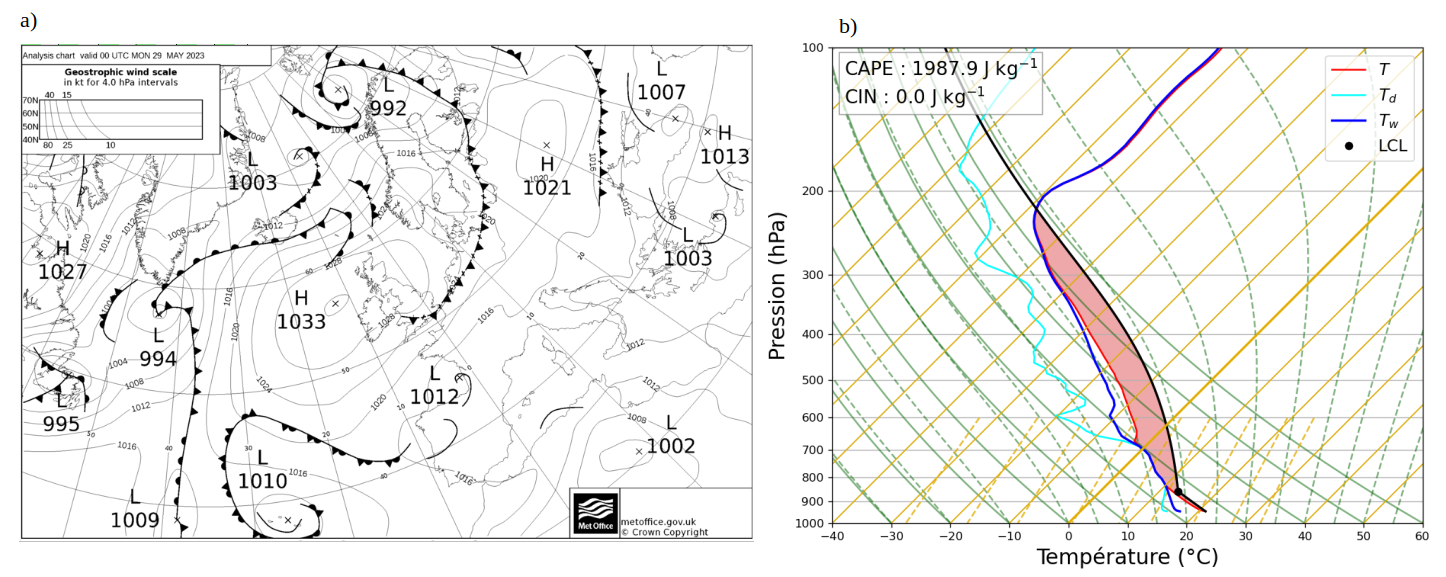
\includegraphics[width=0.9\linewidth]{Sit_Synoptique/Synop.png}
    \caption{a) Analyse météorologique de surface du bureau météorologique britannique le 29 mai 2023 à \protect\nospace{00:00}  UTC. b) Émagramme simulé au-dessus du CRA à \protect\nospace{13:15} UTC.}
    \label{fig:Synop}
\end{figure}
\vspace{-5mm}
\begin{multicols}{2}

\section{Méthodologie}

\subsection{Données à disposition}

Les données d'observation ont été acquises par le satellite Météosat Seconde Génération (MSG) toutes les 15 min, à une résolution de 3 km au nadir, soit environ 4 km à 40°N. La simulation a été effectuée avec le modèle non-hydrostatique de méso-échelle Méso-NH (\cite{lac2018}), développé par Météo-France et le Laboratoire d'Aérologie. Le domaine de simulation est un carré de 512 km de côté, avec une maille de 1 km et centrée sur le CRA de coordonnées 43°07'45.4"N, 0°22'08.0"E. La résolution verticale est 10\,m proche de la surface et décroît jusqu'à valoir 200\,m de 3 à 20\,km au toit du modèle. La simulation est lancée le 29 mai 2023 à \nospace{12:00} UTC à partir de l'analyse ECMWF. Les données de simulation nous sont disponibles de \nospace{13:15} à \nospace{22:00} UTC toutes les 15 min. Elles contiennent les champs 3D atmosphériques (température, vent, contenus en eau) et des images satellites synthétiques de MSG et C2OMODOR calculées avec le code RTTOV. Des variables comme la température potentielle $\theta$ et la température potentielle du thermomètre mouillé $\theta_w$ ont également été utilisées pour la construction de l'émagramme (figure \ref{fig:Synop}). Afin de pouvoir comparer simulation et observation MSG, les données simulées ont été interpolées sur les images MSG. Les principales variables utilisées sont les température de brillance à 10.8 $\mu$m et 325 GHz. Le canal à 10.8 $\mu$m est un canal fenêtre permettant d'observer la température à la surface terrestre, ou en cas de nuages opaques, la température au sommet du nuage. Le canal à 325 GHz est sensible au contenu en vapeur d'eau dans la haute troposphère, ou en cas de nuages convectifs, au contenu en glace de la partie supérieure du nuage. 

\subsection{Algorithme de suivi des cellules}

Le suivi des cellules orageuses a été fait à l'aide d'un algorithme initialement développé pour suivre la croissance des nuages convectifs (\cite{maury}). Ce travail est décomposé en deux étapes : i) l'identification des cellules et ii) leur suivi temporel. La première étape repose sur l'utilisation d'une valeur seuil afin de créer un objet pour chaque cellule. Un objet est un ensemble continu de pixels dont la température de brillance au sommet est inférieure à 220 K. Des tests de sensibilité ont été réalisés avec d'autres valeurs seuils : une valeur plus basse fait  manquer certaines cellules, alors qu'une valeur plus élevée, conduit les objets à s'agglomérer pour n'en former qu'un seul. La deuxième étape repose sur le recouvrement de chaque objet entre les instants $t$ et $t + \Delta t$. L'advection des cellules doit respecter le critère de Courant–Friedrichs–Lewy $(U \Delta t / \Delta x \leqslant 1)$, avec $U$ la vitesse d'advection moyenne à 10 km d'altitude (de l'ordre de 5 m s\textsuperscript{-1}) et $\Delta x$ la maille du domaine. Ainsi, si le nuage se déplace de plus d'une fois sa longueur, la méthode d'identification peut mener à des erreurs. Pour pallier ce problème, seuls les nuages de dimensions supérieures à 3 pixels sont comptabilisés.

\end{multicols}
\vspace{-0.3cm}
\begin{figure}[H]
    \centering
    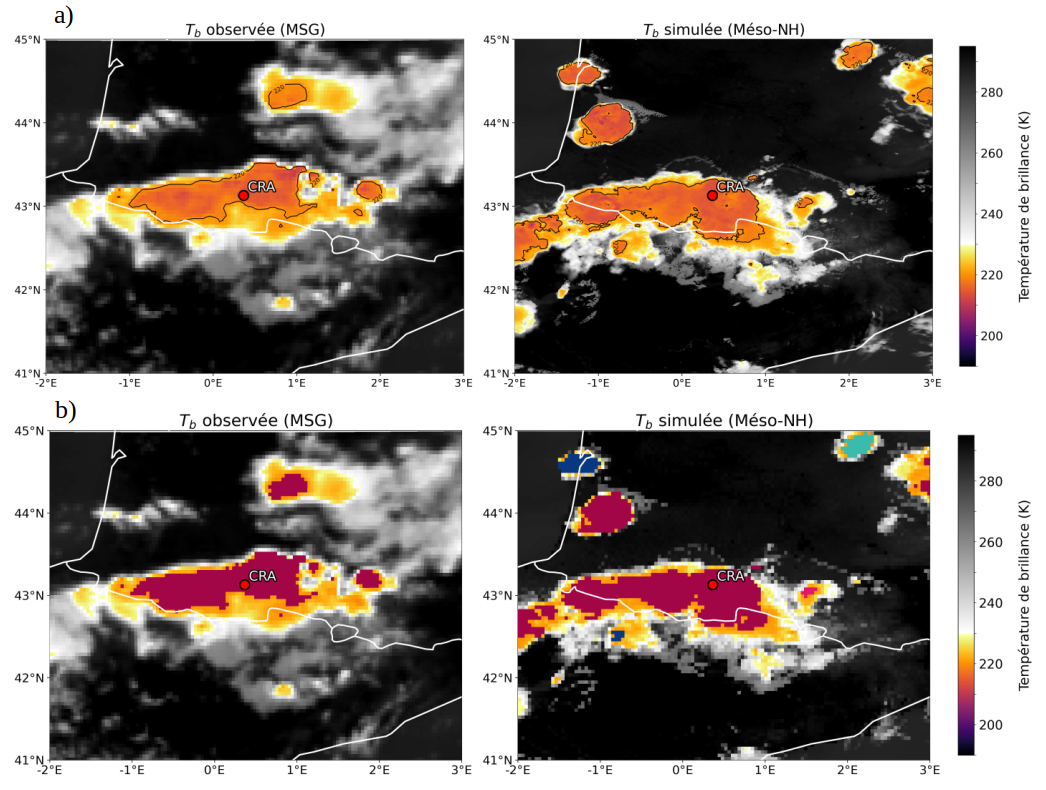
\includegraphics[width=0.8\linewidth]{Figures/Cartes.png}
    \caption{Exemple de comparaisons de cartes de température de brillance à \protect\nospace{16:15} UTC avec à gauche, l'observation et à droite, la simulation. Le CRA est représenté par un rond rouge. a) Données brutes avec une maille de 1 km pour la simulation et l'isotherme 220 K. b) Les cellules de la même couleur font partie du même objet et ont donc un indice unique, ce qui implique qu'ils résultent soit d'une cellule mère qui s'est divisée, soit qu'ils vont fusionner. Les cellules indépendantes ont été numérotées pour plus de clarté. Au total, 2 cellules ont été détectées pour l'observation, et 6 pour la simulation. La grille pour Méso-NH correspond à la grille de MSG.}
    \label{fig:fig2}
\end{figure}

\begin{multicols}{2}

Cet algorithme de suivi permet une continuité temporelle puisque chaque cellule conserve son "indice" au cours du temps. Néanmoins, il a pour faiblesse de considérer chaque cellule amenée à fusionner ou à se diviser comme une seule cellule. Cela explique que plusieurs cellules, à priori isolées sont représentées de la même couleur (figure \ref{fig:fig2}). Un certain nombre de cellules ne sont donc pas comptées en tant que telles dans les analyses ci-après.

Un exemple de sortie de cet algorithme est présenté à \nospace{16:15} UTC. Cet instant a été choisi car il est l'un des plus représentatifs pour la visualisation des résultats. Plus tôt dans l'après-midi, il n'y a pas suffisamment de cellules orageuses et plus tard, les enclumes nuageuses étant bien développées, les cellules s’agrègent et il n'est plus aisé de les distinguer. La simulation retranscrit globalement bien les observations : le système convectif de méso-échelle au-dessus des Pyrénées est déjà bien développé dans les deux cas. Toutefois des différences subsistent dans l'organisation des cellules isolées se trouvant plus au nord. Une seule cellule observée est comptée (numérotée 2) tandis que quatre cellules simulées sont comptées. Certaines d'entre elles se développent un peu plus tard sur l'observation : la dissipation de la cellule 2 vers \nospace{17:00} conduit à la croissance d'une cellule plus importante, à hauteur du bassin d'Arcachon. Ainsi, Méso-NH initie la convection entre 30 min et un heure plus tôt que ce qui a été observé.

\vspace{-3mm}

\section{Résultats et discussion}

\subsection{Comparaison des données du CRA et de simulation}

La vitesse verticale mesurée par le profileur de vent VHF du CRA est comparée à celle simulée au-dessus du CRA (figure \ref{fig:fig3}). A \nospace{15:24} UTC, une ascendance convective est observée avec une vitesse verticale autour de 1–2 m s$^{-1}$ entre 2 et 5 km d’altitude. De \nospace{15:36} à \nospace{16:24} UTC, l’ascendance est confinée au-dessus de 3 km. Elle est la plus intense entre 8 et 10 km d’altitude où des vitesses au-delà de 3 m s$^{-1}$ sont mesurées. Sous cette ascendance, un courant descendant est observé, avec des des vitesses autour de -1 m s$^{-1}$ entre 1.8 et 3 km d’altitude. Cette alternance de vitesses négatives et positives est la signature de cellules en dissipation. De \nospace{16:24} à \nospace{19:48} UTC, la vitesse est le plus souvent négative entre 1.8 et 7 km d’altitude. Ces vitesses négatives correspondent à la partie stratiforme d’un système convectif de méso-échelle et les valeurs les plus basses à 1.8 km d’altitude à la descente de masses d’air refroidi par prélèvement de chaleur latente lors de l'évaporation de la pluie. 

\end{multicols}

\begin{figure}[H]
    \centering
    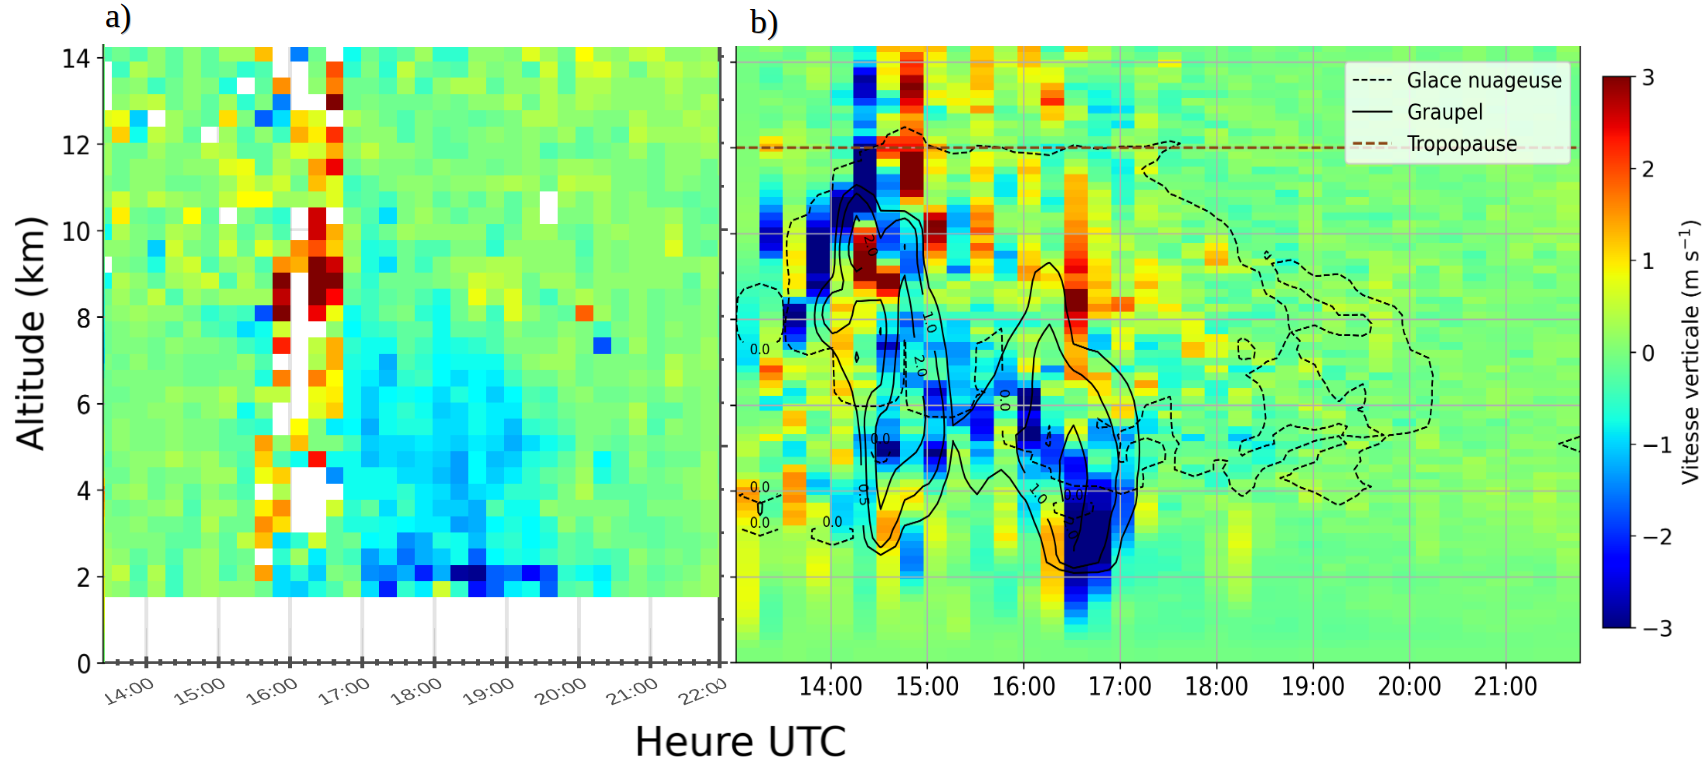
\includegraphics[width=0.9\linewidth]{Figures/CRA_vs_MesoNH.png}
    \caption{Évolution temporelle de la vitesse verticale au-dessus du CRA : a) la vitesse verticale à partir du profileur de vent VHF du CRA moyennée toutes les 12 min (fournie par le CRA et modifiée) et b) la vitesse verticale à partir de la simulation instantanée toutes les 15 min. À droite, le rapport de mélange en graupel en g kg\textsuperscript{-1} est représenté par les iso-contours en noir. L'isoligne 0.01\,g kg\textsuperscript{-1} de glace nuageuse, montrant l'enveloppe nuageuse supérieure est également représentée.}
    \label{fig:fig3}
\end{figure}

\begin{multicols}{2}

La simulation montre une activité convective plus précoce et plus discontinue (figure \ref{fig:fig3}b). Des ascendances de 1-2 m s$^{-1}$ sont ainsi simulées à \nospace{13:15}, \nospace{13:45}, \nospace{14:30} et \nospace{16:15} UTC, entre 1.8 km et jusqu’à 4, voire 7 km. Elles alternent avec des subsidences marquées, jusqu’à -3 m s$^{-1}$, ce qui est caractéristique du passage d'un système convectif de méso-échelle. La précocité de l’activité convective dans la simulation se retrouve sur l’ensemble de la journée (annexe \ref{sec:sec61}). % Des colonnes convectives dépassant les 10 km d'altitude sont également visibles à la fois sur les données VHF et sur la simulation, ce qui peut être la marque des ondes de gravité traversant la tropopause. 
Des vitesses verticales fortes au-dessus de 10 km d'altitude sont également visibles à la fois sur les données VHF et sur la simulation. L'enveloppe nuage simulée jusqu'à 12 km d'altitude nous indique que ces vitesses sont des colonnes convectives en-deça de 12 km et des ondes de gravité au-dessus. L'enveloppe nuageuse dépassant la tropopause située à 12 km à partir de \nospace{14:30} peut être interprétée comme un sommet protubérant.
Les différences d’intensité des vitesses observées et simulées peuvent s’expliquer en partie par leur nature. Les mesures du radar VHF sont moyennées par intervalle de 12 min, alors que les données de la simulation sont des valeurs instantanées obtenues toutes les 15 min. Enfin, le rapport de mélange en graupel, sont des particules de glace précipitantes, de forme conique ou arrondie et d'un diamètre variant de 2 à 5 mm, d'après l'OMM (2024), est également représenté. Les concentrations de graupel les plus élevés se trouvent là où les vitesses verticales sont les plus importantes, tant pour les ascendances que pour les subsidences. 

\subsection{Relation entre la taille de la cellule et \texorpdfstring{$w_{max}$}{TEXT}}
\label{subsec:subsec_w_max}

Des travaux sur le déclenchement de la convection profonde ont proposé une relation implicite pouvait exister entre la taille d'une cellule orageuse et $w_{max}$ (\cite{Rochetin_I}, \cite{Rochetin_II}). Cette relation fait intervenir, entre autres, la racine carrée du logarithme népérien de la section moyenne de la base des ascendances. Bien que la relation proposée par \cite{Rochetin_I} ne fasse pas intervenir directement la surface horizontale de la cellule, il est possible d'y remonter à partir des autres variables à disposition. 

Cette relation a motivé le choix de $w_{max}$ pour caractériser les c\oe urs convectifs bien définis. Avec davantage de temps, une autre approche envisageable aurait été de choisir le quantile 0.975 de la vitesse verticale, par exemple, ce qui aurait appuyé la robustesse statistique en étant moins sensible aux valeurs extrêmes. La variable $w_{max}$ a donc été tracée en fonction de la surface pour les 14 cellules considérées, à chaque pas de temps, soit un total de 209 échantillons. 

En général, $w_{max}$ croît avec la surface de la cellule (figure \ref{fig:W_max_Croissante}). Ce résultat est attendu si on considère que les cellules les plus importantes sont les plus vigoureuses. Cependant, un nombre conséquent de cellules présente des valeurs de vitesse verticale maximum faibles ($ w_{max}<$ 5 m s$^{-1}$) associées à des valeurs de surface très variables (entre 5 et 1000 km\textsuperscript{2}). Une inspection visuelle de ces échantillons nous a conduit à émettre l'hypothèse qu'il s'agissait de cellules en stagnation ou en dissipation, mais rarement en formation. Afin de valider cette hypothèse, les cellules ont été classifiées en 3 catégories : "en croissance", "stable" ou "en dissipation". L'assignation de ces catégories à chaque instant de la cellule est déterminée par l'évolution de sa taille relative au cours du temps : si $(S(t_{i-1}) - S(t_{i+1})) / S(t_{i-1}) > 10 \% $, alors la cellule est qualifiée comme "en croissance". De même, si le précédent rapport est inférieur à $-10 \%$, la catégorie "en dissipation" est assignée à la cellule. Enfin, si ce rapport est compris entre ces valeurs seuils, la cellule est considérée comme stable. Ce critère de classification a été choisi car de nombreux travaux ont mis en avant la relation entre la taille et le cycle de vie de la cellule : une cellule en formation a une taille croissante, et une cellule en dissipation une taille décroissante (\cite{storm_lifecycle1}, \cite{storm_lifecycle2}, \cite{Zobisch}).

Cette classification a permis de mettre en avant deux résultats principaux (figure \ref{fig:wmax_all}). D'une part, les vitesses verticales maximums les plus fortes sont globalement observées pour les cellules en formation. Elles diminuent ensuite au fil de la vie de l'orage. Cela est cohérent avec ce qui est admis aujourd'hui (\cite{Zobisch}). Au stade de cumulus, la vitesse verticale croît avec l'altitude (figure \ref{fig:wt_slice} en annexe). Cela est dû à l'écart de température entre particule d'air ascendante et son environnement qui augmentent avec l'altitude (\cite{Zobisch}). Les vitesses verticales diminuent donc rapidement une fois la phase de croissance achevée à cause du manque de flottabilité. La phase de dissipation est caractérisée par des précipitations, portées par le courant descendant (\cite{Zobisch}).

D'autre part, il a été montré que la relation log-linéaire entre la taille de la cellule et le maximum de vitesse verticale en son sein est plus forte au stade de croissance avec un coefficient de détermination $R^2$ égal à 0.65 (figure \ref{fig:W_max_Croissante}), alors que $R^{2}$ vaut 0.59 et 0.27 aux stades stable et en dissipation, respectivement. Afin d'étudier la corrélation entre la taille de la cellule et $w_{max}$, une étude statistique plus détaillée a été réalisée. Pour choisir le test de corrélation le plus approprié, les tests de Shapiro-Wilk et de Fisher ont été effectués. Le premier permet de tester la normalité de la relation (i.e. si les variables sont distribuées selon une loi normale). Le second permet de vérifier l'égalité des variances entre les deux variables. Les deux tests ne montrant ni normalité ni égalité des variances, le coefficient de corrélation de Spearman associée a été calculé. Ce coefficient représente une mesure de la relation entre deux variables, lorsque la loi de distribution de ces variables est indéterminée (\cite{Spearman}). Enfin, la p-value associée au test de Spearman est également calculée. Cette valeur de juger si la tendance mise en évidence avec le coefficient de corrélation est significative ou non. La p-value étant très inférieure à l'unité, le test de Spearman montre une tendance significative pour une corrélation positive de $w_{max}$ avec la taille de la cellule. Toutes les valeurs obtenues lors de l'analyse statistique de corrélation peuvent être retrouvées dans l'annexe \ref{Annexes:Analyse_stat}.

\vspace{-0.5cm}
\begin{figure}[H]
    \centering
    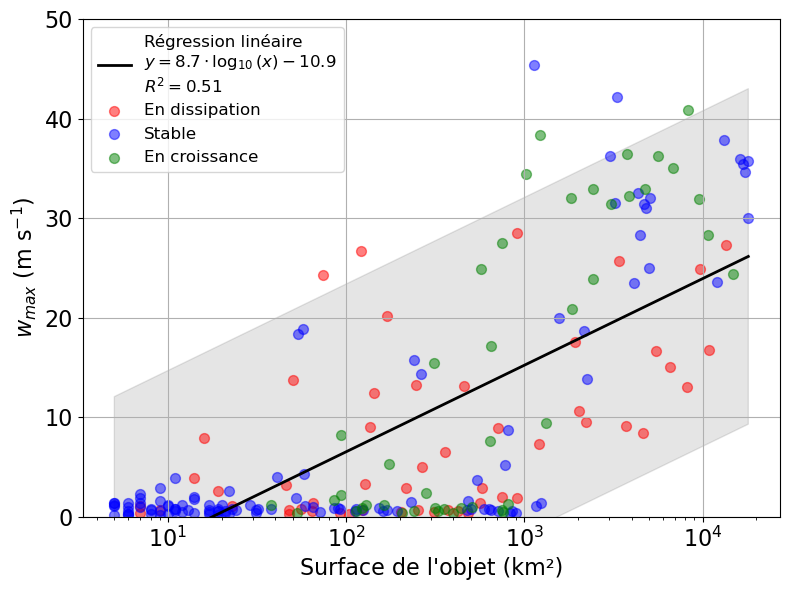
\includegraphics[width=1\linewidth]{Figures/w_max_vs_size.png}
    \vspace{-1em}
    \caption{$w_{max}$ en fonction de la taille de la cellule en considérant l'ensemble des points. Les critères de classification sont détaillés ci-dessous. Pour cette figure ainsi que les figures 5 et 6, la zone grisée correspond à la dispersion au seuil de confiance de 95 \%.}
    \label{fig:wmax_all}
\end{figure}

\vspace{-0.5cm}

Bien que robuste d'un point de vue purement physique, cette méthode admet des aberrations statistiques : des cellules naissantes ou disparaissantes peuvent induire des pourcentages de croissance divergents, puisque leur taille peut être nulle à l'un des deux pas de temps. Néanmoins, cela s'avère être sans conséquence pour les résultats présentés ici, puisqu'il ne s'agit pas d'étudier en détail la distribution de ces pourcentages.

\vspace{-0.5cm}
\begin{figure}[H]
    \centering
    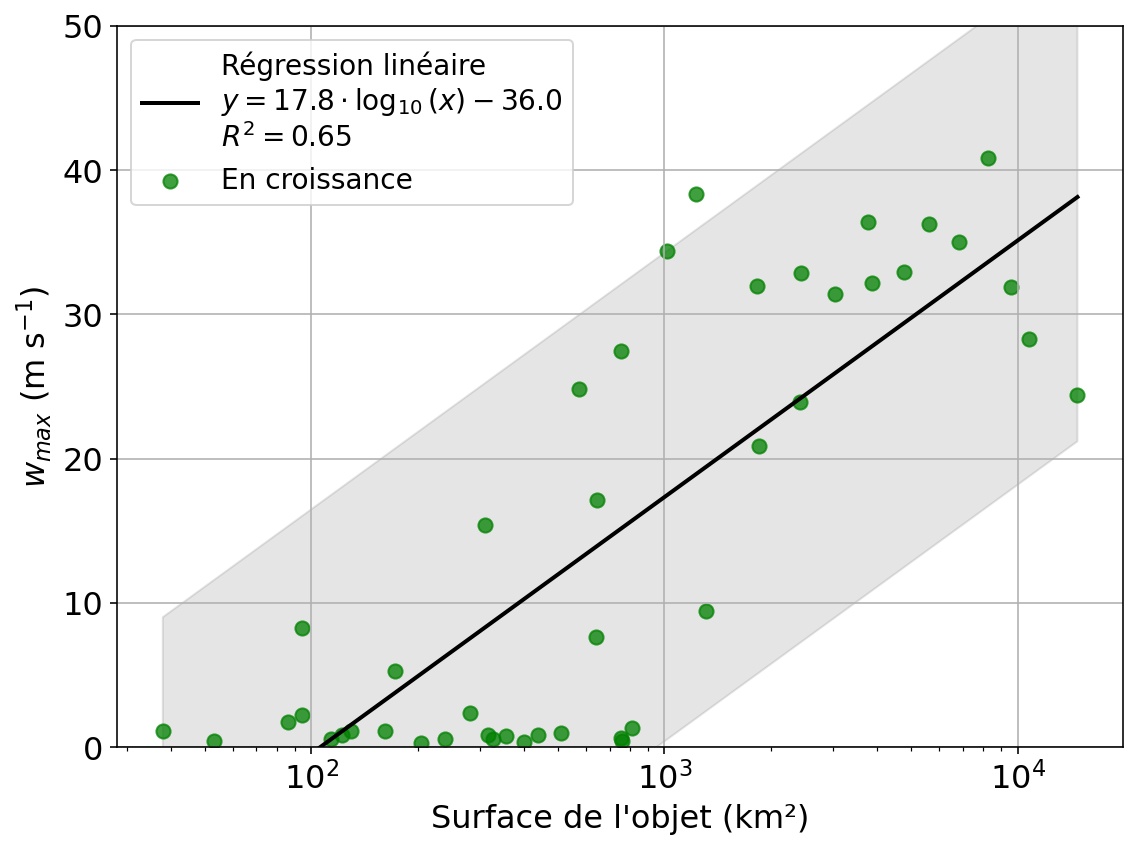
\includegraphics[width=1\linewidth]{Figures/w_max_croissance.png}
    \vspace{-1em}
    \caption{$w_{max}$ en fonction de la taille de la cellule pour le stade de croissance de la cellule convective.}
    \label{fig:W_max_Croissante}
\end{figure}
\vspace{-5mm}
 
\subsection{Relation entre la taille de la cellule et \texorpdfstring{$T_{b, min}$}{TEXT}}

Il a été montré que la température de brillance à 325 GHz et sa dérivée temporelle sont intimement liées au contenu en glace nuageuse (\cite{Chaboureau}). Plus précisément, l'\textit{Ice Water Path} (IWP) croît linéairement avec la dérivée temporelle de la température de brillance $dT_b / dt$, avec :

\begin{equation}
    IWP = \int_z \rho r_{ice} dz
\end{equation}

\noindent où $\rho$ est la masse volumique de l'air en kg\,m$^{-3}$ et $r_{ice}$ le rapport de mélange en glace en kg kg$^{-1}$. 

\begin{figure}[H]
    \centering
    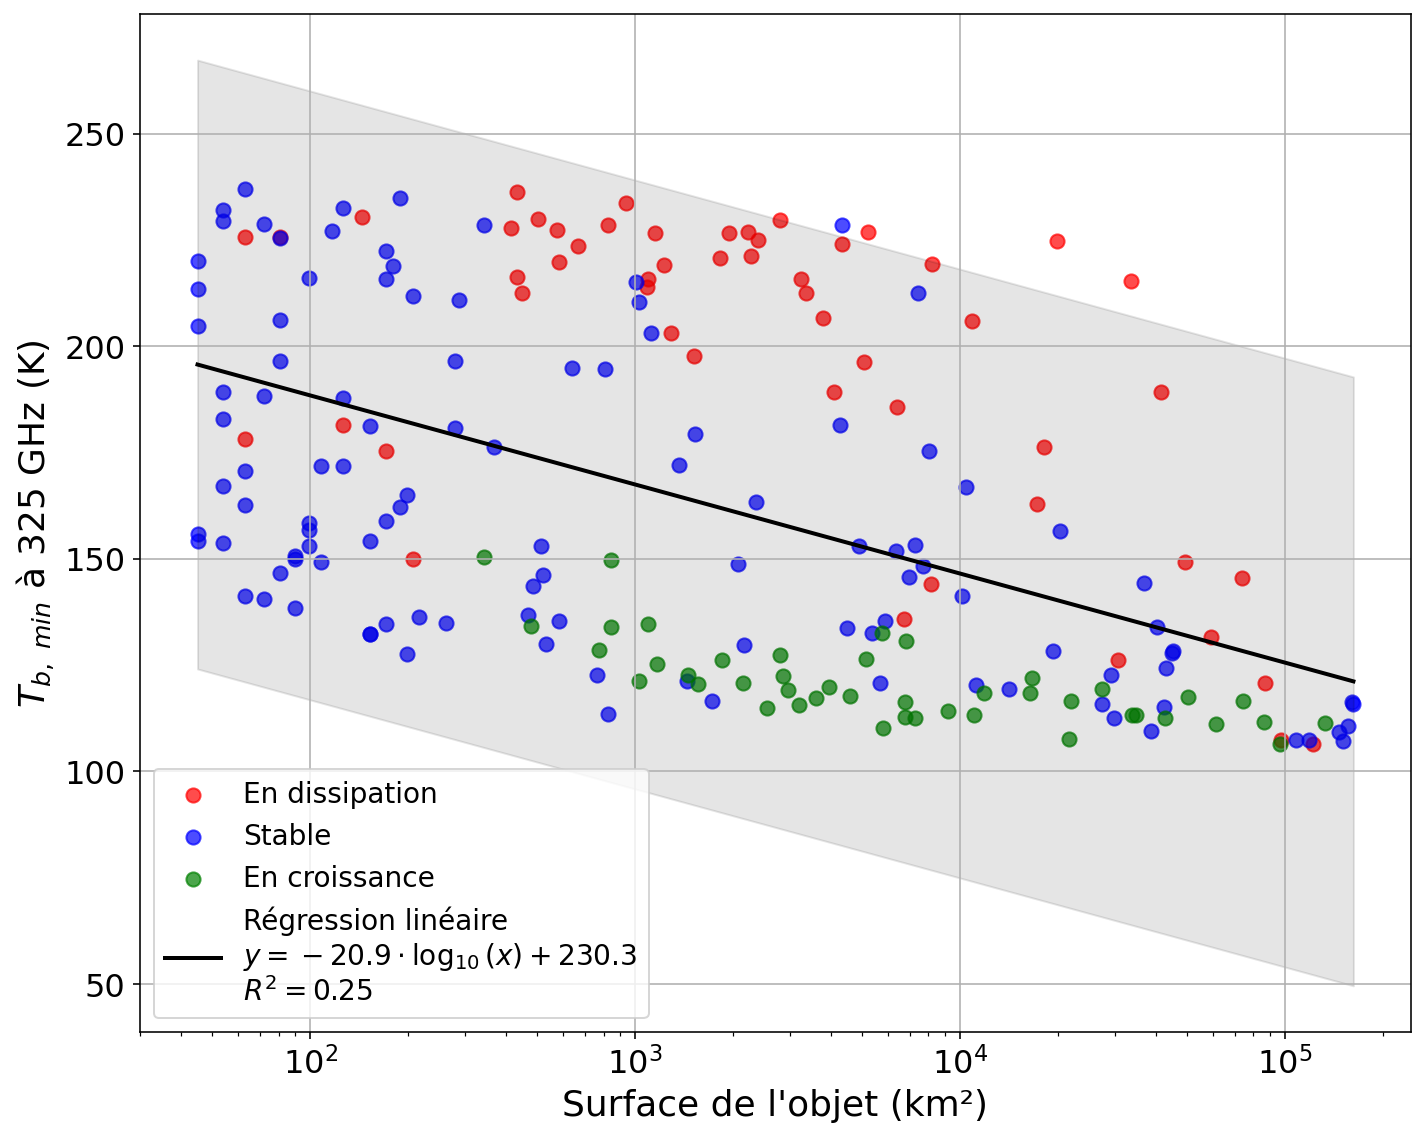
\includegraphics[width=\linewidth]{Figures/min_tb_vs_size.png}
    \caption{Minimum de température de brillance à 325 GHz en fonction du logarithme de la taille de la cellule pour la simulation pour différents stades du cycle de vie des cellules.}
    \label{fig:tb_min_vs_size}
\end{figure}

\vspace{-0.3cm
}
Il est ensuite possible d'avoir accès à la vitesse verticale de la glace à l'aide de la relation suivante :
\vspace{-2mm}
\begin{equation}
    w_{ice} = \frac{VIM}{IWP}
\end{equation}

\noindent où $VIM$ est le \textit{Vertical Ice Momentum} correspondant à l'intégrale sur la verticale du produit $w \times \rho \times r_{ice}$ (\cite{Chaboureau}). L'attention est donc portée sur ce canal. Néanmoins, n'étant pas disponible avec MSG, il ne sera pas possible de confronter les résultats pour l'observation et la simulation pour $T_{b, min}$ à 325 GHz. Les critères de classification pour les cycles de vie des orages sont les mêmes que ceux appliqués dans la Section \ref{subsec:subsec_w_max}. Tout d'abord, $T_{b, min}$ décroît avec la surface de la cellule de façon log-linéaire (figure \ref{fig:tb_min_vs_size}). 

Le coefficient de détermination étant relativement faible pour les cellules qui ne sont pas en stade de croissance, ($R^2_{\text{stabilité}} = 0.33$ et $R^2_{\text{dissipation}} = 0.34$), cette relation n'est pas très forte, du fait d'une dispersion assez importante. Cette tendance est néanmoins significative d'un point de vue statistique, puisque le coefficient de corrélation de Spearman indique une anti-corrélation entre $T_{b, min}$ et la surface de la cellule ($\rho_{\text{croissance}} = -0.753$, $\rho_{\text{stabilité}} = -0.653$ et $\rho_{\text{dissipation}} = -0.816$), avec une p-value très inférieure à l'unité. Ainsi, les cellules dont la température de brillance est la plus faible sont surtout observées au stade de cumulus.

\end{multicols}

\begin{figure}[H]
    \centering
    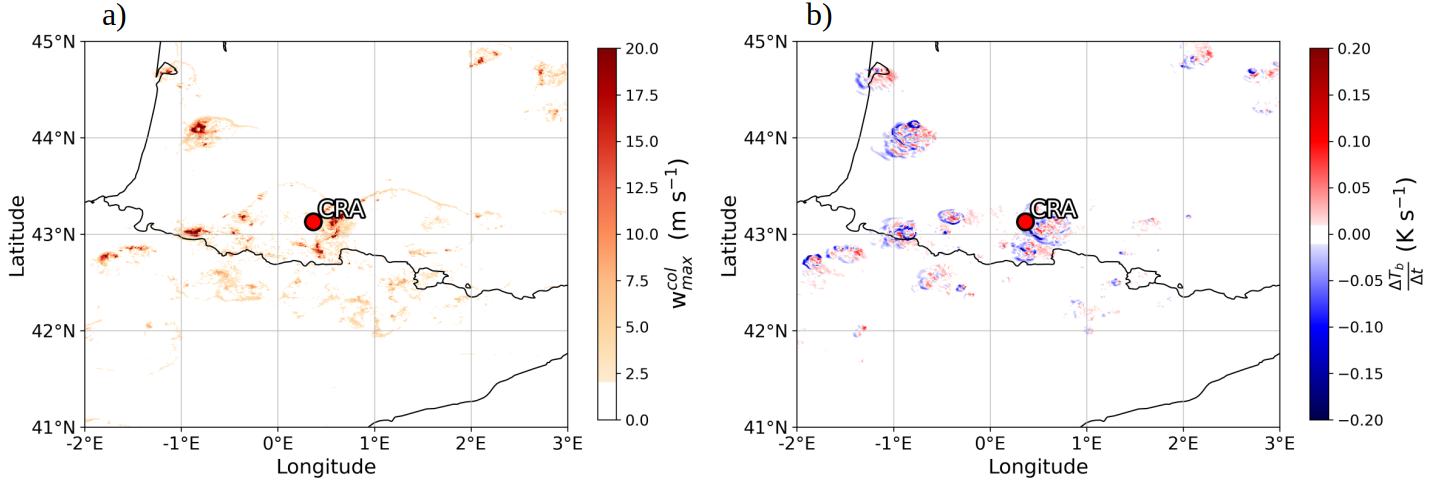
\includegraphics[width=0.9\linewidth]{Figures/deltatb.png}
    \caption{a) Carte de la vitesse maximale par colonne $w_{max}^{col}$ et b) carte de $\Delta T_b / \Delta t$ prises à \protect\nospace{15:45} UTC mettant en évidence les régions de convection profonde : les ascendances fortes sont co-localisées avec les fortes diminutions de la température de brillance à 325 GHz, rappelant ainsi tout l'intérêt de la mission C2OMODO.} 
    \label{fig:delta_tb}
\end{figure}

\begin{multicols}{2}

Cela peut en partie s'expliquer par le fait que c'est au cours de la croissance que les cristaux de glace ont tendance à s'accumuler dans la partie supérieure du nuage, et \textit{a fortiori} dans l'enclume du cumulonimbus. Ainsi la température de brillance augmente lorsque la partie stratiforme se morcelle et que le contenu en glace diminue. 

Ces analyses appuient bien une relation entre la température de brillance (plus spécifiquement sa dérivée temporelle) et la vitesse verticale (\cite{Chaboureau}). Cette relation, attendue pour les c\oe urs convectifs en croissance, peut servir de marqueur de la convection profonde. Les c\oe urs convectifs ayant les plus grandes surfaces sont en général les plus vigoureux, et montrent un contenu en glace et un transport vertical plus importants (figure \ref{fig:delta_tb}). 

\section{Conclusion et perspectives}

Le cas de convection profonde du 29 mai 2023 observé au-dessus du Centre de Recherche Atmosphérique a été étudié à partir des observations satellites MSG, de mesures VHF acquises au CRA, et d'une simulation réalisée avec Méso-NH. La simulation est globalement en accord avec les observations, avec un déclenchement de l'activité orageuse en début d'après-midi dû à une forte instabilité des basses couches. La comparaison des deux séries d'images MSG a néanmoins permis de déceler une avance de la simulation par rapport à la vérité terrain tandis que les vitesses acquises toutes les 12 min au CRA n'ont pas permis de conclure sur le réalisme des vitesses instantanées simulées.

Afin de réaliser un suivi temporel des cellules orageuses, un algorithme de recherche a été utilisé. Ainsi, 14 cellules indépendantes ont ainsi été identifiées, composant un total de 209 échantillons. Cet algorithme n'était sans doute pas le plus adapté à cette étude du fait de sa structure même. En effet, tout ensemble de cellules amenées à se diviser ou \textit{a contrario}, à fusionner est considéré comme une cellule unique. De nombreuses cellules ne sont donc ainsi pas considérées en tant que telles, menant à une perte d'information. La croissance de la vitesse verticale maximum d’une cellule avec sa taille ainsi que sa nature log-linéaire ont pu être mis en évidence dans cette simulation. Les différentes cellules ont été classées en trois catégories au cours de leur cycle de vie. Cette classification est faite selon l’évolution de la taille relative de la cellule, de nombreuses études ayant exhibé une augmentation et une diminution de la taille des cellules orageuses lorsqu’elles sont en croissance et en dissipation, respectivement. La pente de la droite ainsi que la valeur du coefficient de détermination $R^2$ sont d’autant les plus fortes pour les cellules catégorisées comme "en croissance", ce qui est cohérent avec la littérature. Cette relation est donc particulièrement vraie pour les cellules au stade de cumulus.

La variation du minimum de température de brillance à 325 GHz, canal sensible au contenu en glace, a également été examinée en fonction de la taille de la cellule. Dans ce cas, $T_{b, min}$ décroît avec la croissance de la taille. De manière générale, les cellules en croissance présentent les températures de brillance les plus faibles, et celles en dissipation les plus élevées. Cela s’explique par une accumulation des cristaux de glace dans la partie supérieure du nuage, ce qui abaisse la température de brillance. Ces analyses appuient donc la thèse selon laquelle la dérivée temporelle de la température de brillance peut être un puissant indicateur de la croissance des cellules orageuses et par extension, de la vitesse des ascendances. 

Le travail réalisé durant ce stage montre des résultats prometteurs qui demandent cependant des approfondissements. À défaut de pouvoir disposer d'une mesure VHF à haute fréquence d'échantillonnage, la vitesse verticale simulée nécessite d'être moyennée sur 12 min afin de pouvoir comparer à la mesure. Le suivi des cellules appelle à l'utilisation d'un algorithme plus adapté, notamment capable de considérer la fusion et la division des cellules. Les relations entre la surface de la cellule et, vitesse verticale maximum ou minimum de température de brillance, ont été obtenues pour un échantillon limité en nombre. Il serait donc très intéressant d’examiner ces relations pour d’autres simulations afin de vérifier que plus la cellule orageuse sera grande, plus la mesure de sa vitesse depuis l’espace sera facilitée.
 
\end{multicols}

\clearpage
\vspace*{-2cm}
\section{Annexes}

\subsection{Analyse des critères de Pone} \label{Pone}

Les données de la simulation ont été utilisées pour tracer un émagramme au-dessus du CRA, afin d'étudier la stabilité de l'atmosphère avant le déclenchement de l'orage (\nospace{13:15} UTC). Pour réaliser l'analyse des critères de Pone, les couches atmosphériques ont été divisées de la façon suivante: \\

\begin{itemize}
    \item \textbf{1000 à 850 hPa} : du sol jusqu'au niveau de condensation (LCL pour Lifting Condensation Level).
    \item \textbf{850 à 704 hPa} : du LCL jusqu'au sommet de la couche instable. 
    \item \textbf{704 à 300 hPa} : du sommet instable jusqu'au début d'une autre couche saturée. 
    \item \textbf{300 à 200 hPa} : jusqu’au dépassement du niveau d’équilibre thermique (LNB pour Level of Neutral Buoyancy).  \\  
\end{itemize}

Dans chaque couche, les évolutions de la température potentielle ($\theta$) et de la température pseudo-adiabatique du thermomètre mouillé ($\theta_w$) ont été notées.

\subsubsection*{1000 à 850 hPa : $\theta \searrow$ ; $\theta_w \searrow$ } 

Une diminution de $\theta$ et $\theta_w$ a été observée le long de la couche, ce qui correspond à un cas d'instabilité absolue. Cette couche est initialement non saturée et instable, mais avec une humidité relative élevée, caractérisée par le rapprochement de la courbe d'état avec la courbe de température de rosée. Lorsque la masse d'air est soulevée de 150 hPa, la couche devient saturée, en étant toujours instable. 

\subsubsection*{850 à 704 hPa : $\theta \nearrow$ ; $\theta_w \searrow$}

Bien que la tendance à la diminution de $\theta_w$ soit maintenue, $\theta$ diminue, ce qui indique que cette couche est dans un cas d'instabilité convective, plus précisément, un cas d'instabilité convective sélective. En effet, le LCL se trouve à l'intérieur de la couche. Puisque le niveau de saturation est atteint, la présence de nuages cumuliformes est certaine.  

La base du nuage est localisée au LCL qui est aussi la basse de la couche, située à 857 hPa, et son sommet moyen ($S_{moyen}$) à la fin de cette couche, où la courbe d'état s'incline à droite des adiabatiques. 

\subsubsection*{704 à 300 hPa : $\theta \nearrow$ ; $\theta_w \nearrow$}

Au regard de la croissance de $\theta$ et $\theta_w$, cette couche est absolument stable. Cette couche étant non saturée, les nuages présents sont ceux formés dans les couches inférieures, et qui se sont développés jusqu'à atteindre ce niveau.

\subsubsection*{300 à 200 hPa : $\theta \nearrow$ ; $\theta_w \nearrow$}

 Toujours en présence d'une augmentation de $\theta$ et $\theta_w$ la couche est elle aussi absolument stable. Il est possible d'y observer le LNB, et donc le sommet maximal ($S_{max}$) des nuages cumuliformes formé dans les bases couches plus instables. \\

\noindent L'emplacement des nuages à partir de cet analyse peut être trouvé dans la figure \ref{fig:analyse_pone}.

\begin{figure}[H]
    \centering
    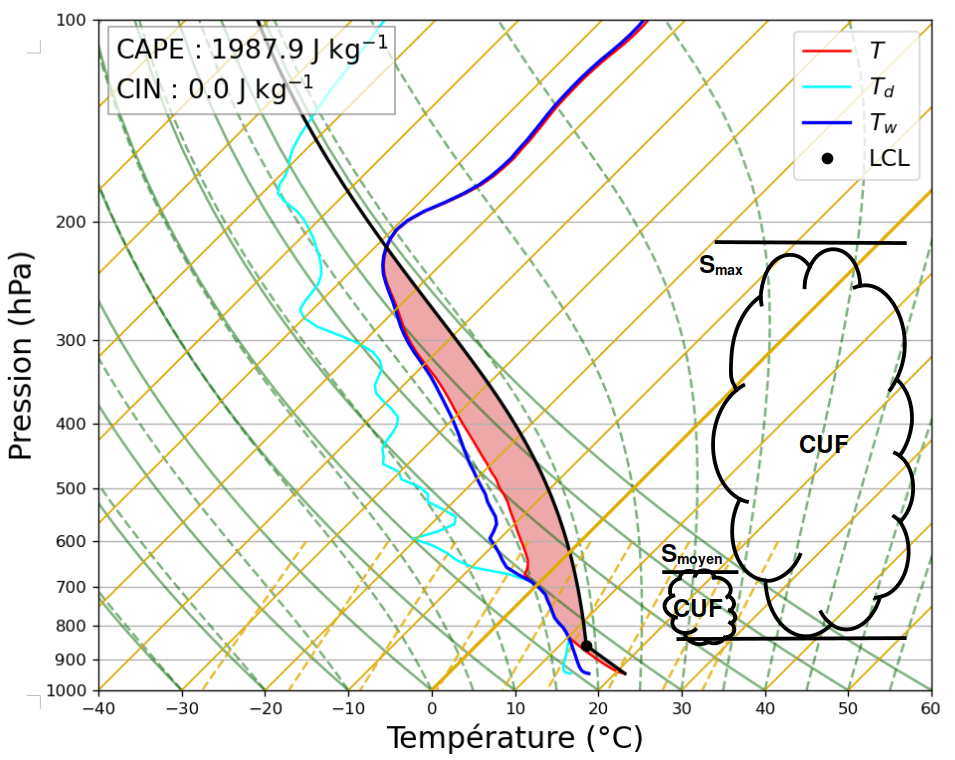
\includegraphics[width=0.8\linewidth]{Figures/Analyse_Emagramme.png}
    \caption{Figure \ref{fig:Synop} - b) avec les niveaux nuageux déterminés à l'aide des critères de Pone.}
    \label{fig:analyse_pone}
\end{figure}

\newpage

\subsection{Exemple de suivi temporel des cellules}
\label{sec:sec61}

\vspace{-0.7cm}

\begin{figure}[H]
    \centering
    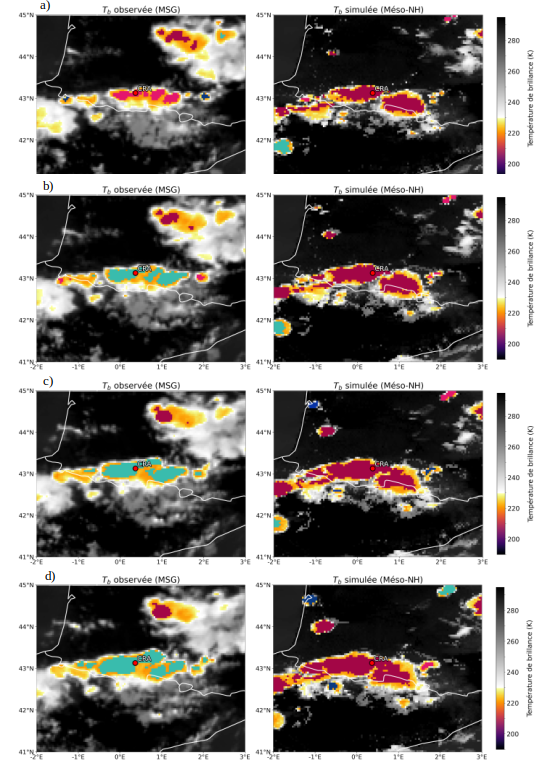
\includegraphics[width=0.9\linewidth]{Figures/suivi_temporel.png}
    \caption{Exemple de sorties pour le suivi temporel des cellules orageuses avec, à gauche, l'observation MSG et à droite, la simulation Méso-NH (dégradée). En toute rigueur, les cellules de la même couleur font partie du même objet. Des incohérences peuvent néanmoins apparaître, comme c’est le cas entre \protect\nospace{13:15} et \protect\nospace{15:15} UTC pour l'amas nuageux au centre des images MSG.}
    \label{fig:suivi_temporel}
\end{figure}

\newpage

\subsection{Résultats des analyses statistiques}
\label{Annexes:Analyse_stat}

\subsubsection*{$w_{max}$ en fonction de la taille de la cellule}

\begin{table}[H]
    \centering
    \resizebox{\textwidth}{!}{%
    \begin{tabular}{||l||p{2.5cm}||p{2.5cm}||p{2.5cm}||}
    \hline
        \textbf{Paramètre} & \textbf{Croissance} & \textbf{Stabilité} & \textbf{Dissipation} \\ \hline \hline
        $R^2$ & 0.65 & 0.59 & 0.27 \\ \hline 
        Moyenne  & 14.69 & 7.24 & 8.04\\ \hline
        Écart-type  & 14.86 & 12.20 & 8.60 \\ \hline
        %Intercept & -36.0 & -9.9 & -4.6 \\ \hline
        Coefficient de Shapiro-Wilk & 0.80 & 0.61 & 0.83\\ \hline
        Coefficient de Fisher &  0.38 & 1.67 & 1.00 \\ \hline
        Coefficient de Spearman & 0.72 & 0.52 & 0.51 \\ \hline
    \end{tabular}%
    }
    \label{tab:Stat_Wt_max}
\end{table}



\subsubsection*{$T_{b, min}$ en fonction de la taille de la cellule (canal 325 GHz)}

\begin{table}[H]
    \centering
    \resizebox{\textwidth}{!}{%
    \begin{tabular}{||l||p{2.5cm}||p{2.5cm}||p{2.5cm}||}
    \hline
        \textbf{Paramètre} & \textbf{Croissance} & \textbf{Stabilité} & \textbf{Dissipation} \\ \hline \hline
        $R^2$ & 0.52 & 0.33 & 0.34 \\ \hline 
        Moyenne  & 120.62 & 162.23 & 197.47 \\ \hline
        Écart-type  & 9.69 & 37.58 & 36.72 \\ \hline
        %Intercept & 159.85 & 221.29 & 281.93 \\ \hline
        Coefficient de Shapiro-Wilk & 0.89 & 0.33 & 0.34 \\ \hline
        Coefficient de Fisher & 1.30 & 0.45 & -1.01 \\ \hline
        Coefficient de Spearman & -0.75 & -0.56 & -0.54 \\ \hline
    \end{tabular}%
    }
    \label{tab:Stat_Tb_min_325}
\end{table}

\subsection{Coupes de vent vertical}
\label{sec:secwt}

\begin{figure}[H]
    \centering
    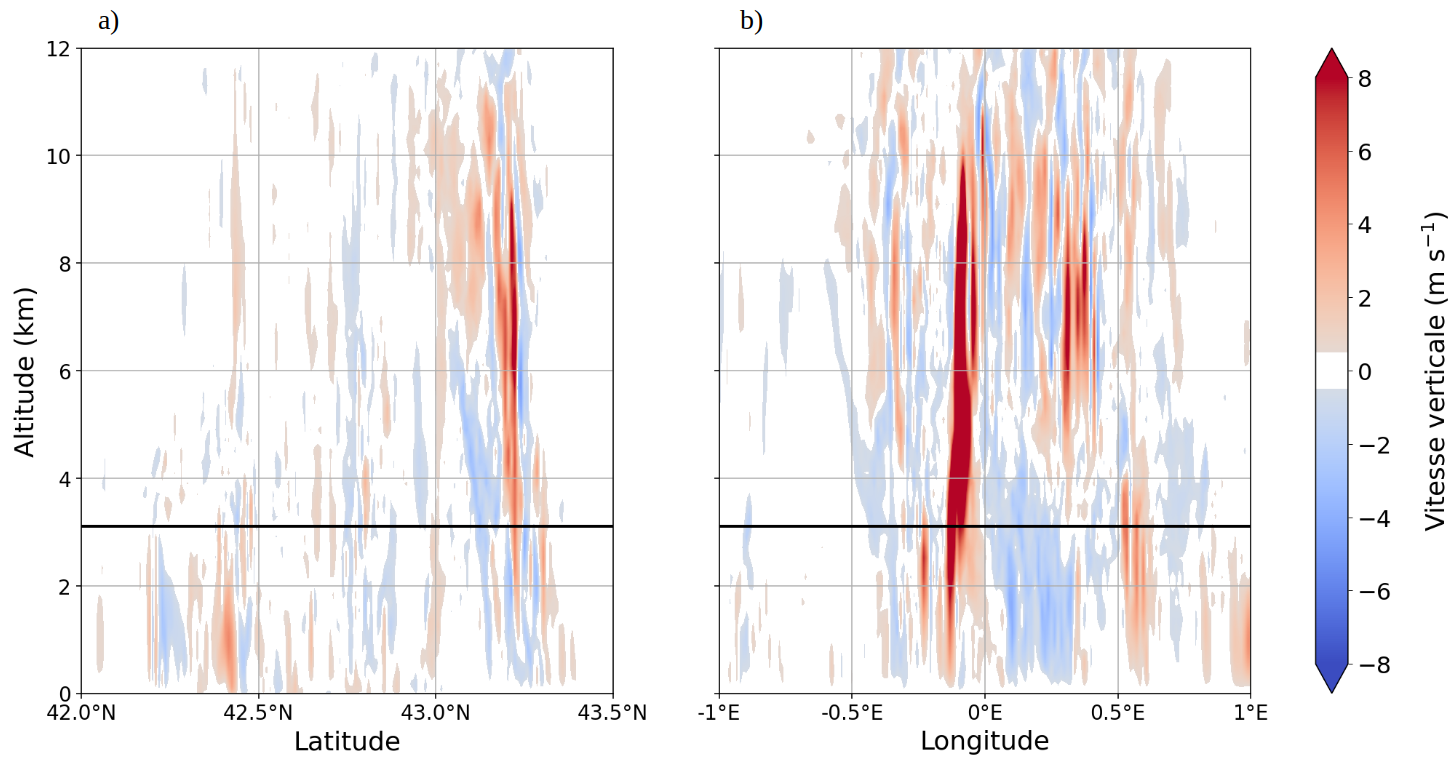
\includegraphics[width=0.9\linewidth]{Figures/vertical_wt_slice.png}
    \caption{Coupes verticale a) N-S et b) E-O de vitesse verticale passant par le CRA à \protect\nospace{15:15} UTC. L'isotherme 0°C au-dessus du CRA  est également représenté, ce qui montre que les vitesses verticales sont généralement plus élevées au-dessus du niveau de congélation.}
    \label{fig:wt_slice}
\end{figure}

\newpage    
\nocite{*}
\printbibliography[title = {Références}]

\noindent Lien GitHub vers le code utilisé : \url{https://gitlab.com/tropics/objects/}
\end{document}

